\documentclass{acm_proc_article-sp}

\usepackage{multirow}
\usepackage{rotating}
\usepackage{color}
\usepackage{pdfcolmk}

\newcommand{\col}[1]{{\color{red} #1}}
\newcommand{\cod}[1]{\hspace{0.1cm}\texttt{#1}}
\newcommand{\ing}[1]{\emph{#1}}
\newcommand{\preempt}{{Preempt-RT}}
\newcommand{\preemptt}{{Preempt-RT }}

\usepackage[font=normalsize, justification=Centering, singlelinecheck=false]{my_caption}
\usepackage[captionskip=1pt]{my_subfig}
%\renewcommand{\captionfont}{\sffamily\small\bfseries}


\begin{document}

% \usepackage{graphicx,url}

% \usepackage[brazil]{babel} \usepackage[latin1]{inputenc}

     
%\sloppy
 
\title{Evaluation of Interrupt Handling Timeliness\\in Real-Time Linux Operating Systems}

\numberofauthors{3}
\author{
\alignauthor
Paul Regnier\\%\titlenote{Dr.~Trovato insisted his name be first.}\\
       \affaddr{Distributed Systems Laboratory (LaSiD)}\\
       \affaddr{Computer Science Department (DCC)}\\
%       \affaddr{Campus de Ondina, 40170-110, Salvador-BA, Brazil}\\
       \affaddr{Federal University of Bahia}\\
       \email{pregnier@ufba.br}
%
\alignauthor
George Lima \\%\titlenote{Dr.~Trovato insisted his name be first.}\\
       \affaddr{Distributed Systems Laboratory (LaSiD)}\\
       \affaddr{Computer Science Department (DCC)}\\
%       \affaddr{Campus de Ondina, 40170-110, Salvador-BA, Brazil}\\
       \affaddr{Federal University of Bahia}\\
       \email{gmlima@ufba.br}
%
\alignauthor
Luciano Barreto \\%\titlenote{Dr.~Trovato insisted his name be first.}\\
       \affaddr{Distributed Systems Laboratory (LaSiD)}\\
       \affaddr{Computer Science Department (DCC)}\\
%       \affaddr{Campus de Ondina, 40170-110, Salvador-BA, Brazil}\\
       \affaddr{Federal University of Bahia}\\
       \email{lportoba@ufba.br}
}

\date{30 July 1999}


\maketitle
%\begin{multicols}{2}

\begin{abstract}
  Several real-time Linux extensions are available nowadays. Two of those extensions
  that have received special attention recently are Preempt-RT and Xenomai. This
  paper evaluates to what extent they provide deterministic guarantees when reacting
  to external events, an essential characteristic when it comes to real-time
  systems. For this, we define two simple experimental approaches.  Our results
  indicate that Preempt-RT is more prone to temporal variations than Xenomai when
  the system is subject to overload scenarios.
\end{abstract}
      
\category{D.4.8}{Operating Systems}{Performance}[Measurements]

\terms{Measurement, Performance}

\keywords{Real Time, Interrupt Handling, Operating System, Linux}%NOT required for Proceedings


\section{Introduction}

Real-time systems encompasses a broad range of applications in multimedia,
transportation, manufacturing, telecommunications, health etc. In all these
scenarios, correctly choosing a Real-Time Operating System (RTOS) is a fundamental
design issue. Although technological hardware advances are essential to the
development of the IT industry, some of these innovations may introduce undesirable
unpredictability to the implementation of a RTOS. For example, cache memories,
direct memory access, out-of-order execution and branch prediction units may
introduce non-negligible sources of indeterminism \cite{Liu00, Pratt04}. Thus, the
construction of a general purpose operating system with focus on timing
predictability remains a challenging research issue.

Although Linux is a popular and widely used OS, the standard Linux kernel
\cite{Bovet05} fails to provide the timing guarantees required by critical real-time
systems \cite{Marchesotti06, Abeni02}. To circumvent this problem, several
approaches have been developed in order to increase the timing predictability of
Linux \cite{PreemptRT, Xenomai, Dozio03, Barabanov97, Fry07, Calandrino06}. The
diversity and constant evolution in their design call for comparative studies to
assess the determinism degree offered by such platforms. The results of this kind
of studies can help real-time systems designers to choose the appropriate solution
according to their needs.

This paper presents and compares two real-time Linux kernel patches, \preemptt
(Linux$^{\mathbf{Prt}}$) \cite{PreemptRT} and Xenomai \linebreak \noindent
(Linux$^{\mathbf{Xen}}$) \cite{Xenomai}, developed to increase the predictability of
Linux. The main contributions of this work are: (i) an evaluation procedure based on
simple software and COTS hardware, and (ii) a report analysis of \preemptt and
Xenomai latency performance obtained through our experimental results. Overall,
these results show that Linux$^{\mathbf{Xen}}$ provides better timing guarantees
than Linux$^{\mathbf{Prt}}$.

The remainder of this paper is structured as follows. Section \ref{sec:irqHand}
introduces some basic definitions and discusses some sources of unpredictability in
Linux. Then, both Linux$^{\mathbf{Prt}}$ and Linux$^{\mathbf{Xen}}$ are described.
The metrics used in our evaluation are also defined in this section. Section
\ref{sec:metod} describes our experiments and results are given in Section
\ref{cap:platEstud}. Finally, Section \ref{sec:trabRel} briefly discusses related
work and Section \ref{sec:conc} concludes the paper. 

\section{Interrupt Handling}
\label{sec:irqHand}

An \textbf{interrupt request} (IRQ) of the processor is typically asynchronous and
can happen at any time during the processor execution cycle. After being issued by a
hardware device or a software exception, an interrupt request is eventually detected
by the processor. When it occurs, the detection of an IRQ diverts the processor to a piece
of code outside the on-going execution flow. Such a code is called \textbf{interrupt
  handler} or interrupt service routine (ISR).

In this work, we call both an interrupt request and its related interrupt handler
execution as \textbf{interruption}. We say that interruptions are disabled when
the processor is not allowed to divert its on-going execution flow to the code of an
interrupt handler.

It is important to note that the asynchronous nature of interrupt requests implies
that they can occur while the critical section of another interrupt handler is
already being executed by the processor, possibly with interruptions disabled. This
scenario may delay the detection of interrupt requests by the processor in a
non-deterministic manner. The way the OS handles interruptions implies its
predictability level.


\subsection{Linux}
\label{sec:linuxStd}

The conventional method used to minimize the impact of interruptions on the response
time of processes is to divide the implementation of interrupt handlers into two
parts. The first part, referred to as the \textbf{critical section} of the handler,
runs critical operations immediately after its activation, usually with
interruptions disabled.  One may enable interruptions during some parts of a
critical section in order to enable preemptions. However, such an implementation
must rely on locks to ensure controlled access to shared data. The second part of
the handler is dedicated to non-critical operations. Its execution can be delayed
and normally happens with interruptions enabled.  In Linux, this second part of the
handlers are called \textbf{\emph{softirqs}}.

Just after the end of the critical section of an interrupt handler, the associated
\emph{softirq} becomes able to be executed. However, between the instant at which
the critical section execution terminates and the instant at which the deferred
\emph{softirq} begins to execute, other interruptions may occur, causing a possible
delay in starting the \emph{softirq} execution. These possible extra delays have direct
impact on real-time operating systems, where timeouts or hardware events are used to
trigger tasks, in a similar manner as \emph{softirqs}.


\subsection{Linux Preempt-RT}
\label{sec:preemptRT}

Linux$^{\mathbf{Prt}}$ \cite{McKenney05, Rostedt07} is a Linux real-time patch
originally developed by Ingo Molnar.  This patch makes the Linux kernel almost fully
preemptible by re-engineering the use of locks inside the kernel.  As soon as a high
priority process is released, it can acquire the processor with low latency, with no
need to wait for the end of the execution of a lower priority process, even if such
a process is running in kernel mode. Also, in order to limit the unpredictability
caused by shared resources, Linux$^{\mathbf{Prt}}$ provides synchronization
primitives that are able to use a priority inheritance protocol
\cite{Sha90}. Further, a specific implementation of high resolution timers
  \cite{Kernel} allows the kernel to provide time resolution in the order of
  microseconds. For instance, using such timers, other researchers \cite{Rostedt07,
    Siro07} were able to measure latencies with an accuracy of the order of $\mu
  s$.

Linux$^{\mathbf{Prt}}$ creates specific kernel threads to handle both software and
hardware interrupt requests.  Upon an IRQ, the associated handler masks the request,
wakes up the associated thread and returns to the interrupted code. This
  approach greatly reduces the execution latency of the critical part of interrupt
  handlers in comparison with the standard Linux approach. The interrupt thread
that has been woken up is eventually scheduled according to its priority and then
starts executing.  Another advantage of Linux$^{\mathbf{Prt}}$ is that several Linux
legacy software packages such as C libraries and programming environments can be
used.

\pagebreak
It is interesting to note that the threaded implementation of interrupt handlers in
Linux$^{\mathbf{Prt}}$ may be a source of unpredictability when interrupt threads
are delayed by the scheduling policy or by other interrupt requests. Nevertheless,
Linux$^{\mathbf{Prt}}$ offers the option \cod{IRQF\_NODELAY} which allows one to
disable the threaded implementation of a specific interrupt line. When this option
is set, interrupts are handled as in standard Linux.

\subsection{Linux Xenomai}
\label{sec:xenomai}

Xenomai or Linux$^{\mathbf{Xen}}$ is a real-time Linux framework that encompasses an
OS kernel, APIs and a set of utilities. It uses an interrupt request indirection
layer \cite{Stodolsky93}, also called nanokernel, to isolate real-time tasks from
Linux processes. According to this approach, when an IRQ occurs, the nanokernel
forwards the request either to a real-time task or to a conventional Linux
process. In the first case, the interrupt handler runs immediately. In the second
case, the request is enqueued and is further delivered to Linux when there are no
more pending real-time tasks. Whenever the Linux kernel requests disabling
interruptions, the nanokernel just makes the Linux kernel believe that interruptions
are disabled. The nanokernel keeps intercepting any hardware interrupt requests.
The interrupt requests targeted to Linux are kept enqueued until the Linux kernel
requests enabling interruptions.

The nanokernel of Linux$^{\mathbf{Xen}}$ is based on a resource virtualization layer
called Adeos (Adaptative Domain Environment for Operating Systems)
\cite{Yaghmour01}. Adeos eases hardware sharing and provides a small API which is
architecture independent. In short, Adeos relies on two basic concepts: domains and
hierarchical interrupt pipelines. A domain defines an isolated execution
environment, according to which one can run programs or even a complete operating
system. The hierarchical interrupt pipeline, called \textbf{ipipe}, delivers 
interrupt request across different domains. When a domain is registered, it is
stored in a specific position in the ipipe according to its timing requirements. The
interrupt indirection mechanism handles hierarchical IRQ deliveries following
the priority associated to each domain.

Real-time services in Linux$^{\mathbf{Xen}}$ correspond to the highest priority
domain in the ipipe, which is called the primary domain. The secondary domain refers
to the Linux kernel itself, from which common Linux software libraries are
available. At this level, however, Linux$^{\mathbf{Xen}}$ offers weaker timing
guarantees due to the way user process are mapped into kernel threads.

\subsection{Evaluation metrics}
\label{sec:evalMetrics}

Clearly, the way interrupt handlers are dealt with by an OS kernel interferes in the
system timeliness as a whole.  In this paper, we consider two metrics to analyze the
timing behavior of an OS: interrupt latency and activation latency.

\subsubsection*{Interrupt latency}
\label{sec:latIRQ}

This first metric is directly induced by the interruption mechanism explained
earlier in this section. Thus, the \textbf{interrupt latency} is defined as the
time interval between the instant at which an interrupt request is issued and the
starting time of the execution of the associated handler.

\begin{figure*}[t!]
  \centering {\scalebox{1}{\input{fig/dispExp.pstex_t}}}
  \caption{Interrupt and activation latencies at station $E_M$ for the
    first experiment}
  \label{fig:dispExp}
\end{figure*}

\subsubsection*{Activation latency}

To define this second metric, we considered a real-time task $\tau$ which is
suspended while waiting for an event. When such event occurs, the associated
interrupt request triggers the corresponding handler which, in turn, wakes up
$\tau$.  Thus, the \textbf{activation latency}, is defined as the time interval
between the instant of the event occurrence and the consequent beginning execution 
of $\tau$.

As for \emph{softirqs}, the activation latency may be increased by the occurrence of
interruptions. Furthermore, the execution of other \emph{softirqs} may be scheduled
according to some policy (eg FIFO, fixed priority), which can also generate
interference in the activation latency. 


\section{Case studies}
\label{sec:metod}

In general, performing accurate time measurements at the interruption level is
not simple and may require the use of external devices such as oscilloscopes or
other computers. In fact, the exact instant at which an interrupt request occurs is
difficult to be determined since this is an asynchronous event which can be
triggered by any hardware device. Nevertheless, since the objective of this work is
to characterize and compare the degree of predictability in different operating
systems platforms, we adopt simple experiment setups that is easily reproducible.
In other words, we are interested in measuring approximate values of latencies for
different real-time OS under similar load scenarios.
 
To compare the OS platforms two experiments were set up, both of which use
only computer stations connected to each other by standard communication
devices. These two experiments, described in Sections \ref{sec:exp1} and
\ref{sec:exp2}, are to measure interrupt and activation latencies with and without
load scenarios.  These latencies are denoted $L_{irq}$ and $L_{act}$,
respectively. The procedure to generate load scenarios is given in Section
\ref{sec:carga}. 

One may choose only one of these two experiments. The first is simpler and can
be used for comparison purpose. The second is more elaborated and provides
more accurate measurements of interrupt latencies.

\subsection{First experiment}
\label{sec:exp1}

\begin{figure}[h]
  \centering {\scalebox{0.67}{\input{fig/config.pstex_t}}}
  \caption{First experiment setup}
  \label{fig:config}
\end{figure}

Figure \ref{fig:config} illustrates how the first experiment was set up. We use 
three stations, $S_T$, $S_L$ and $S_M$ and two distinct Ethernet
network devices, $eth_0$ and $eth_1$, to connect $S_T$ to $S_M$ and $S_L$
to $S_M$, respectively. The role of $S_T$ is to \emph{trigger} events at the
parallel port of $S_M$. Such events should be timely handled by $S_M$, the station
whose latencies are \emph{measured}.  $S_L$ is the \emph{load} station, used to
create load scenarios on $S_M$ via $eth_1$, as will be explained in Section
\ref{sec:carga}.

The activities handled by $S_M$ are illustrated in Figure \ref{fig:dispExp}. The
following sequence of events occurs:

%\pagebreak
\begin{enumerate}
\item $S_T$ sends Ethernet frames to $S_M$, which are received through its $eth_0$
  device. Upon the receiving of each frame the device $eth_0$ issues an interrupt
  request at $S_M$. In turn, the associated interrupt handler (ISR$_{eth_0}$) preempts
  the application that is executing on $S_M$.

\item ISR$_{eth_0}$ triggers an interrupt request on the Parallel Port (PP)
    interrupt line and saves the instant $t_1$ in memory.  Note that $t_1$ is the
  local time at $S_M$ and is read just after the arrival of an Ethernet frame at
  $eth_0$.

\item Upon the detection of the parallel port interrupt request, its handler
  ISR$_{PP}$ preempts the application on $S_M$.  Then ISR$_{PP}$ saves the instant
  $t_2$ and wakes up task $\tau$. This second time instant is the local time value
  at $S_M$ just after the start of ISR$_{PP}$.
  
\item When task $\tau$ wakes up, it saves instant $t_3$ in memory and then is
  suspended until the next PP event. Thus, $t_3$ is the time instant at which
  $\tau$ starts executing.
\end{enumerate}

During the experiment runs, the measured values of $L_{irq}$ and $L_{act}$ were
transferred from main memory to a file system in $S_M$ by a user process using a FIFO
channel. The assigned priority of the user process was lower than the priority of
interrupt handlers.  Also, this data transferring procedure generated sufficiently rare
events (20 per second). This data transferring scheme was to prevent possible
interference in the measured values.

In order to compare the behavior of the analyzed platforms, both latencies can be
computed by the described procedure as $L_{irq} = t_2 - t_1$ and $L_{act} = t_3 -
t_2$, as depicted in Figure \ref{fig:dispExp}. However, it is worth noticing that
the measurements are performed by the same station that is responsible for managing
real-time activities. Indeed, station $S_M$ waits for the asynchronous arrival of an
Ethernet frame at $eth_0$ to trigger the corresponding parallel port interrupt
request so that measurements can be carried out. This dependence between external
and internal events may compromise some measurements. In order to evaluate to what
extent such a procedure interfere in the measurements, a second experiment was set
up.

\begin{figure*}[t]
  \centering {\scalebox{1}{\input{fig/dispExp2.pstex_t}}}
  \caption{Interrupt and activation latencies measurement at station $S_M$ for the
    second experiment}
  \label{fig:dispExp2}
\end{figure*}

\subsection{Second experiment}
\label{sec:exp2}

The same three stations $S_M$, $S_T$ and $S_L$ are used in this experiment
setup. Station $S_L$ is configured as before while the other 
two stations have different roles, as shown in Figure~\ref{fig:config2}.

%\afterpage{\clearpage}
\begin{figure}[htb]
  \centering {\scalebox{0.67}{\input{fig/config2.pstex_t}}}
  \caption{Second experimental set-up}
  \label{fig:config2}
\end{figure}


Similar to the first experiment, the values of $L_{irq}$ and $L_{act}$ correspond to
real-time activities executed by $S_M$. However, the measurements are carried out by
$S_T$ instead. The measurement procedure makes use of the parallel port that
connects $S_T$ and $S_M$, as can be seen from the figure.  The device $eth_0$ is no
longer necessary.  In other words, station $S_T$ triggers PP interrupt requests at
$S_M$ via its parallel port. Station $S_M$ handles such interrupt requests, waking
up a real-time task $\tau$ similarly to the previous experiment.

Note that in this second experiment, measurements could not be carried out by $S_M$
unless station local clocks were synchronized to each other. To avoid dealing with
extra complication due to clock synchronization protocol, time measurements are
performed only at $S_T$.  For example, suppose that the time occurrence of an event
$e$ on $S_M$ needs to be measured. In such a case, just after $e$,
$S_M$ triggers back an interrupt request on the $S_T$ PP interrupt line and the
measurement is taken at $S_T$ while this interrupt request is handled by ISR$_{PP}$.
As a consequence, the described measurement procedure must take into account the
interrupt latency $\delta$ in $S_T$. In other words, if $e$ occurs at real-time $t$
on $S_M$, it will be measured at real-time $t+ \delta$ on $S_T$.

The value of $\delta$ can be estimated, for example, by carrying out the first
experiment, but without using station $S_L$. In this work, we used
Linux$^{\mathbf{Xen}}$ at $S_T$, running in single mode with minimal load. The
estimated value of $\delta$ was taken as the mean value $\bar{\delta}$ observed in
the measurements obtained with the first experiment. For this platform
$\bar{\delta} = 9 \mu s$ with standard deviation $0.1 \mu s$.

% Once this estimation was obtained, the operating system
%   patch in $S_T$ must be fixed so that $\bar{\delta}$ can be used as an accurate
%   estimation of $\delta$ during the experiments.  }

Figure \ref{fig:dispExp2} summarizes the sequence of events that occur in $S_M$ and
$S_T$, which makes up the second measurement procedure:

\begin{enumerate}
\item Station $S_T$ triggers an interrupt request on the PP interrupt line of
  station $S_M$ and saves instant $t_1$ in memory. This time instant is the local
  clock of $S_T$ just after the interrupt is requested.
 
\item The PP interrupt request (PP-IRQ) is detected by the $S_M$ processor and
    the ISR$_{PP}$ handler of $S_M$ is activated, causing the preemption of the
    application running on $S_M$.

\item The handler ISR$_{PP}$ of $S_M$ triggers back an interrupt request on
  the PP interrupt line of station $S_T$ and wakes up task $\tau$.
  
\item The PP-IRQ is detected by the $S_T$ processor and the PP interrupt handler
    ISR$_{PP}$ of $S_T$ saves time $t_2$ in memory.  This time instant corresponds
    to the value of the local clock of $S_T$ just after the start of its ISR$_{PP}$.
  
\item Task $\tau$ wakes up in $S_M$ and triggers back a new interrupt request on the
  PP interrupt line of station $S_T$.
  
\item The handler ISR$_{PP}$ of $S_T$ is activated to deal with this second interrupt
  request, saving the current value of its local clock $t_3$. This instant
  corresponds to the time at which $S_T$ is informed about the activation of $\tau$.
\end{enumerate}

As can be seen from Figure \ref{fig:dispExp2}, differently from the first
experiment, now $L_{irq} = t_2 - t_1 - \delta$.  On the other hand, some care must
be taken in order to measure $L_{act}$ accurately as the interrupt request issued by
$\tau$ may take place before or after $t_2$, introducing an experimental variability
not related to the real value of $t_3 - t_2$. This issue will be further discussed
when analyzing the obtained experimental results in Section \ref{cap:platEstud}.

During the measurements, the obtained values were transferred from memory to a file
system in $S_T$ using the same data transferring scheme used in the first
experiment. In order to minimize any possible interference, $S_T$ was run in single
user mode with minimal load.

\subsection{Load scenarios}
\label{sec:carga}

The experiments were carried out with and without load scenarios in station
$S_M$. Without any load, $S_M$ was set up with its kernel in single mode and with
minimum activities, i.e. both $S_L$ and no other process in $S_M$ generate extra
load. As will be seen, in general, the analyzed real-time patches present high
levels of predictability under this situation.

The load generated was applied to station $S_M$, which was stressed by two different
types of load, triggered by internal and external events. Both types of load were
started a few seconds before the beginning of the measurements.  As will be
seen, under such load scenarios, it was possible to assess to what extent the
analyzed real-time patches can provide predictability.

The internal events that generated CPU and I/O load on $S_M$ were performed by
executing the following shell commands:

\framebox[0.47\textwidth]{%
  \begin{minipage}{0.84\linewidth}
    \vspace{2pt } \scriptsize{%
      \texttt{while "true"; do\\
        \rule{0.3cm}{0pt} dd if=/dev/hda2 of=/dev/null bs=1M count=1000\\
        \rule{0.3cm}{0pt} find / -name "*.c" | xargs egrep include\\
        \rule{0.3cm}{0pt} tar -cjf /tmp/root.tbz2 /usr/src/linux-xenomai\\
        \rule{0.3cm}{0pt}  cd /usr/src/linux-preempt; make clean; make\\
        done \vspace{2pt } %\nolinebreak %\raisebox{10mm}{\rule{0cm}{0.01cm}}
      }}
  \end{minipage}
}

The external events used to load $S_M$ were due to the arrival of 64 byte UDP
packets at $eth_1$ sent by station $S_L$. Station $S_M$ was configured as a server
and $S_L$ as a client. The packet sending rate was set to $200 kHz$, which is the
maximum network rate allowed. With this setup, we were able to issue more than
$100,000$ interrupt requests per second at $eth_1$. This device used $S_M$ interrupt
line $18$, whose priority is lower than the priority of the PP interrupt line. Thus,
in an ideal situation, one would expect that receiving packets from $eth_1$ would
not interfere in the execution of PP interrupt request related events.

\section{Results}
\label{cap:platEstud}

The experiments were conducted on three Pentium 4 computers with $2.6 GHz$
processors and $512 MB$ RAM memory. Three operating system platforms were analyzed,
one of which with two configuration options:

\begin{description}
\item[$\bullet \;$ Linux$^{\mathbf{Std}}$:] Linux standard - kernel version 2.6.23.9
  (\ing{low-latency} option);
\item[$\bullet \;$ Linux$^{\mathbf{Prt}}$:] Linux with \ing{patch}
  \preemptt (rt12) - kernel version 2.6.23.9;
\item[$\bullet \;$ Linux$^{\mathbf{PrtND}}$:] Linux$^{\mathbf{Prt}}$ with option
  \cod{IRQF\_NODELAY} used to initialize the PP interrupt line;
\item[$\bullet \;$ Linux$^{\mathbf{Xen}}$:] Linux with \ing{patch} Xenomai - version
  2.4-rc5 - kernel version 2.6.19.7.
\end{description}

Linux$^{\mathbf{Std}}$ was considered for the sake of illustration. Although this
general purpose OS is not suitable to deal with real-time applications, it has been
used here as a reference, against which one can compare real-time Linux
patches. Linux$^{\mathbf{PrtND}}$ corresponds to setting the option
\cod{IRQF\_NODELAY} at the initialization time of PP interrupt line. As seen in
Section \ref{sec:preemptRT}, using this option, interrupt handling of that line is
implemented without threads.  Latencies $L_{irq}$ and $L_{act}$ were measured using
the Time Stamp Counter (TSC), which provided a precision of less than $30 ns$ (88
cycles) in our tests.  As mentioned earlier, station $S_T$ was used to trigger
$20Hz$ events at station $S_M$.  The measured data were the result of running the
experiments for ten minutes for each experiment type and platform.

Experimental results are presented through graphs in which the horizontal axes
represent the instant at which the latencies were measured, which ranges from 0 to
60 seconds.  The vertical axes represent the measured latencies in $\mu s$. These
values can be multiplied by $2.6\:10^3$ to obtain the corresponding number of TSC
cycles.  Values outside the vertical axis range are represented by a triangle near
the maximum value.  Below each graph the following values are given: Mean (M),
Standard Deviation (SD), minimum (Mn) and maximum (Mx). These numbers were obtained
considering the duration of ten minutes of each experiment run. Although each
experiment was run for ten minutes, one-minute time window was found sufficient to
illustrate the timing behavior of each platform.  During this time interval, the
total number of events is $1\,200$ as the arrival frequency of Ethernet frames at the
$eth_0$ network device of station $S_M$ is $20 Hz$.

We first present in Section \ref{sec:results-1} the results from the first
experiment.  Then, in Section \ref{sec:results-2}, we analyze the procedure
suggested by the second experiment. Section \ref{sec:compTable} discusses the
results obtained by these two experiments.
%\newline

\subsection{First Experiment}
\label{sec:results-1}

For the sake of illustration, we first discuss the results regarding
Linux$^\mathbf{Std}$.  Then, we present the measurements obtained for the other
platforms.

\subsubsection*{Linux$^\mathbf{Std}$}

As can be seen from Figure \ref{fig:latIrq-std}, the obtained values without load
show that interrupt handling in Linux is reasonably efficient. As it will be seen
shortly, these values are very close to some RTOS platforms.  However, both
$L_{irq}$ and $L_{act}$ vary significantly in the presence of load, as
expected.  In particular, the obtained values of $L_{act}$ in load scenarios
confirm that Linux$^\mathbf{Std}$ is not suitable to support real-time systems.
Indeed, the maximum value of $L_{act}$ was found to be about 17 times the mean value.

%\newpage
\begin{figure*}[t!]%
% \centering
 \subfloat[\small{\textbf{Linux$^{\mathbf{Std}}$ - Interrupt latency - without load} \newline
 \vskip 1mm M:     8.9, SD:     0.3,  Mn:     8.7, Mx:    18.4 }]{%
   \label{fig:ker23Sem}%
   {\scalebox{0.67}{\input{fig/ker23Sem}}}} \hspace{10pt}%
 \subfloat[\small{\textbf{Linux$^{\mathbf{Std}}$ - Interrupt latency - with load} \newline
 \vskip 1mm M:    10.4, SD:     1.9,  Mn:     8.8, Mx:    67.7 }]{%
   \label{fig:ker23Tot}%
   {\scalebox{0.67}{% GNUPLOT: LaTeX picture with Postscript
\begingroup
  \makeatletter
  \providecommand\color[2][]{%
    \GenericError{(gnuplot) \space\space\space\@spaces}{%
      Package color not loaded in conjunction with
      terminal option `colourtext'%
    }{See the gnuplot documentation for explanation.%
    }{Either use 'blacktext' in gnuplot or load the package
      color.sty in LaTeX.}%
    \renewcommand\color[2][]{}%
  }%
  \providecommand\includegraphics[2][]{%
    \GenericError{(gnuplot) \space\space\space\@spaces}{%
      Package graphicx or graphics not loaded%
    }{See the gnuplot documentation for explanation.%
    }{The gnuplot epslatex terminal needs graphicx.sty or graphics.sty.}%
    \renewcommand\includegraphics[2][]{}%
  }%
  \providecommand\rotatebox[2]{#2}%
  \@ifundefined{ifGPcolor}{%
    \newif\ifGPcolor
    \GPcolorfalse
  }{}%
  \@ifundefined{ifGPblacktext}{%
    \newif\ifGPblacktext
    \GPblacktextfalse
  }{}%
  % define a \g@addto@macro without @ in the name:
  \let\gplgaddtomacro\g@addto@macro
  % define empty templates for all commands taking text:
  \gdef\gplbacktext{}%
  \gdef\gplfronttext{}%
  \makeatother
  \ifGPblacktext
    % no textcolor at all
    \def\colorrgb#1{}%
    \def\colorgray#1{}%
  \else
    % gray or color?
    \ifGPcolor
      \def\colorrgb#1{\color[rgb]{#1}}%
      \def\colorgray#1{\color[gray]{#1}}%
      \expandafter\def\csname LTw\endcsname{\color{white}}%
      \expandafter\def\csname LTb\endcsname{\color{black}}%
      \expandafter\def\csname LTa\endcsname{\color{black}}%
      \expandafter\def\csname LT0\endcsname{\color[rgb]{1,0,0}}%
      \expandafter\def\csname LT1\endcsname{\color[rgb]{0,1,0}}%
      \expandafter\def\csname LT2\endcsname{\color[rgb]{0,0,1}}%
      \expandafter\def\csname LT3\endcsname{\color[rgb]{1,0,1}}%
      \expandafter\def\csname LT4\endcsname{\color[rgb]{0,1,1}}%
      \expandafter\def\csname LT5\endcsname{\color[rgb]{1,1,0}}%
      \expandafter\def\csname LT6\endcsname{\color[rgb]{0,0,0}}%
      \expandafter\def\csname LT7\endcsname{\color[rgb]{1,0.3,0}}%
      \expandafter\def\csname LT8\endcsname{\color[rgb]{0.5,0.5,0.5}}%
    \else
      % gray
      \def\colorrgb#1{\color{black}}%
      \def\colorgray#1{\color[gray]{#1}}%
      \expandafter\def\csname LTw\endcsname{\color{white}}%
      \expandafter\def\csname LTb\endcsname{\color{black}}%
      \expandafter\def\csname LTa\endcsname{\color{black}}%
      \expandafter\def\csname LT0\endcsname{\color{black}}%
      \expandafter\def\csname LT1\endcsname{\color{black}}%
      \expandafter\def\csname LT2\endcsname{\color{black}}%
      \expandafter\def\csname LT3\endcsname{\color{black}}%
      \expandafter\def\csname LT4\endcsname{\color{black}}%
      \expandafter\def\csname LT5\endcsname{\color{black}}%
      \expandafter\def\csname LT6\endcsname{\color{black}}%
      \expandafter\def\csname LT7\endcsname{\color{black}}%
      \expandafter\def\csname LT8\endcsname{\color{black}}%
    \fi
  \fi
  \setlength{\unitlength}{0.0500bp}%
  \begin{picture}(7200.00,5040.00)%
    \gplgaddtomacro\gplbacktext{%
      \csname LTb\endcsname%
      \put(1034,594){\makebox(0,0)[r]{\strut{}$0.0$}}%
      \put(1034,1117){\makebox(0,0)[r]{\strut{}$5.0$}}%
      \put(1034,1640){\makebox(0,0)[r]{\strut{}$10.0$}}%
      \put(1034,2162){\makebox(0,0)[r]{\strut{}$15.0$}}%
      \put(1034,2685){\makebox(0,0)[r]{\strut{}$20.0$}}%
      \put(1034,3208){\makebox(0,0)[r]{\strut{}$25.0$}}%
      \put(1034,3731){\makebox(0,0)[r]{\strut{}$30.0$}}%
      \put(1034,4253){\makebox(0,0)[r]{\strut{}$35.0$}}%
      \put(1034,4776){\makebox(0,0)[r]{\strut{}$40.0$}}%
      \put(1166,374){\makebox(0,0){\strut{}$ 0$}}%
      \put(2109,374){\makebox(0,0){\strut{}$ 10$}}%
      \put(3053,374){\makebox(0,0){\strut{}$ 20$}}%
      \put(3996,374){\makebox(0,0){\strut{}$ 30$}}%
      \put(4939,374){\makebox(0,0){\strut{}$ 40$}}%
      \put(5883,374){\makebox(0,0){\strut{}$ 50$}}%
      \put(6826,374){\makebox(0,0){\strut{}$ 60$}}%
      \put(396,2685){\rotatebox{90}{\makebox(0,0){\strut{}Lat\^encia em $\mu s$}}}%
      \put(3996,110){\makebox(0,0){\strut{}Tempo de observa\c{c}\~ao em $s$}}%
    }%
    \gplgaddtomacro\gplfronttext{%
    }%
    \gplbacktext
    \put(0,0){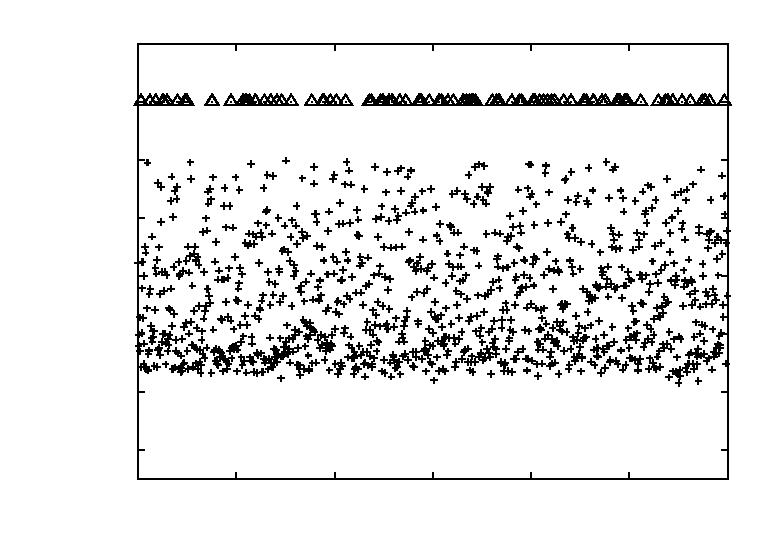
\includegraphics{fig/ker23Tot}}%
    \gplfronttext
  \end{picture}%
\endgroup
}}}%
   
 \subfloat[\small{\textbf{Linux$^{\mathbf{Std}}$ - Activation latency - without load} \newline
 \vskip 1mm M:     4.6, SD:     0.4,  Mn:     4.4, Mx:    16.2}]{%
   \label{fig:ker23SemSched}%
   {\scalebox{0.67}{\input{fig/ker23SemSched}}}} \hspace{10pt}%
 \subfloat[\small{\textbf{Linux$^{\mathbf{Std}}$ - Activation latency - with load}\newline
 \vskip 1mm M:    37.3, SD:    48.2,  Mn:     4.6, Mx:   617.5}]{%
   \label{fig:ker23TotSched}%
   {\scalebox{0.67}{\input{fig/ker23TotSched}}}}
   
 \caption[Linux$^{\mathbf{Std}}$ latencies]{Linux$^{\mathbf{Std}}$ latencies.  The
   $eth_0$ interrupt handler is triggered by packets arriving at a $20 Hz$ frequency.}
 \label{fig:latIrq-std}%
\end{figure*}


\subsubsection*{Linux$^\mathbf{Prt}$, Linux$^\mathbf{PrtND}$ and
  Linux$^\mathbf{Xen}$}

Figures \ref{fig:latIrq} and \ref{fig:latAtiv} plot the values of $L_{irq}$ and
$L_{act}$, respectively.  Six graphs are shown in each Figure. The right and left
columns show results with and without load, respectively.

As for the interrupt latencies (see Figure \ref{fig:latIrq}), Linux$^{\mathbf{Xen}}$
clearly shows higher predictability when compared to the other platforms. Under load
scenarios, this behavior is evident as it can be noticed by the lower mean and
standard deviation values. In order to explain the behavior of
Linux$^{\mathbf{Prt}}$, some aspects need to be explained.  First, when
\cod{IRQF\_NODELAY} is set, the behavior of Linux$^{\mathbf{Prt}}$ turns to be
similar to Linux$^{\mathbf{Std}}$, although Linux$^{\mathbf{Prt}}$ exhibits better
results. On the other hand , using threads for interrupt handling increases the
interrupt latency due to an extra context-switching overhead.  Also, a significantly
higher variability on latency values happens when the system is overloaded. This can
be explained by the execution delay of the handler.  Indeed, between the instant at
which ISR$_{PP}$ issues the interrupt and the instant at which the IRQ thread actually
wakes up, several interrupts may occur.  In such a scenario, the execution of
related interrupt handlers may delay the execution of ISR$_{PP}$.

\begin{figure*}[t!]%
 \centering
 \subfloat[\small{\textbf{Linux$^{\mathbf{Prt}}$ - without load} \newline
 \vskip 1mm M: 21.5, SD: 1.7, Mn: 20.3, Mx: 45.1 }]{%
   \label{fig:preSem}%
   {\scalebox{0.67}{\input{fig/preSem}}}} \hspace{10pt}%
 \subfloat[\small{\textbf{Linux$^{\mathbf{Prt}}$ - with load} \newline
 \vskip 1mm M: 58.5, SD: 26.4, Mn: 17.2, Mx: 245.9}]{%
   \label{fig:preTot}%
   {\scalebox{0.67}{\input{fig/preTot}}}} \vspace{14pt}%

 \subfloat[\small{\textbf{Linux$^{\mathbf{Prt}}$ - without load, option
     \cod{IRQF\_NODELAY}} \newline
   \vskip 1mm M: 8.9, SD: 0.2, Mn: 8.8, Mx: 16.7}]{%
   \label{fig:preSemND}%
   {\scalebox{0.67}{\input{fig/preSemND}}}} \hspace{10pt}%
 \subfloat[\small{\textbf{Linux$^{\mathbf{Prt}}$ - with load, option
     \cod{IRQF\_NODELAY}} \newline
   \vskip 1mm M: 10.6, SD: 1.6, Mn: 8.9, Mx: 35.8}]{%
   \label{fig:preTotND}%
   {\scalebox{0.67}{\input{fig/preTotND}}}}  \vspace{14pt}%

 \subfloat[\small{\textbf{Linux$^{\mathbf{Xen}}$ - without load} \newline
 \vskip 1mm M: 9.0, SD: 0.1, Mn: 8.8, Mx: 11.1}]{%
   \label{fig:xenSem}%
   {\scalebox{0.67}{\input{fig/xenSem}}}} \hspace{10pt}%
 \subfloat[\small{\textbf{Linux$^{\mathbf{Xen}}$ - with load} \newline
 \vskip 1mm M: 10.2, SD: 0.1, Mn: 8.8, Mx: 20.8}]{%
   \label{fig:xenTot}%
   {\scalebox{0.67}{\input{fig/xenTot}}}}  \vspace{14pt}%

 \caption[Interrupt latencies]{Interrupt latencies. The
   $eth_0$ interrupt handler is triggered by packets arriving at a $20 Hz$ frequency.}
 \label{fig:latIrq}%
\end{figure*}

Figure \ref{fig:latAtiv} shows activation latencies with and without load.  It is
worth noting the behavior of Linux$^{\mathbf{Prt}}$ and Linux$^{\mathbf{Xen}}$ with
load. Despite the mean value found for Linux$^{\mathbf{Xen}}$ ($8,7 \mu s$) is
greater than the one found for Linux$^{\mathbf{Prt}}$ ($3,8 \mu s$), the standard
deviation is significantly lower in favor of Linux$^{\mathbf{Xen}}$. In fact, this
is a desirable feature in hard real-time systems. Additionally, for such systems, it
is desirable that the worst-case execution time be as close as possible to the
average-case execution time.
     
      
       
\begin{figure*}[t!]%
 \centering
 \subfloat[\small{\textbf{Linux$^{\mathbf{Prt}}$ - without load} \newline
 \vskip 1mm M: 2.1, SD: 0.2, Mn: 1.2, Mx: 9.4}]{%
   \label{fig:preSemSched}%
   {\scalebox{0.67}{\input{fig/preSemSched}}}} \hspace{10pt}%
 \subfloat[\small{\textbf{Linux$^{\mathbf{Prt}}$ - with load} \newline
 \vskip 1mm M: 3.8, SD: 2.8, Mn: 1.1, Mx: 27.4}]{%
   \label{fig:preTotSched}%
   {\scalebox{0.67}{\input{fig/preTotSched}}}}  \vspace{14pt}%

 \subfloat[\small{\textbf{Linux$^{\mathbf{Prt}}$ - without load, option
     \cod{IRQF\_NODELAY}} \newline
 \vskip 1mm M:     5.3, SD:     0.3,  Mn:     5.0, Mx:    13.1}]{%
   \label{fig:preSemSchedND}%
   {\scalebox{0.67}{\input{fig/preSemSchedND}}}} \hspace{10pt}%
 \subfloat[\small{\textbf{Linux$^{\mathbf{Prt}}$ - with load, option
     \cod{IRQF\_NODELAY}} \newline
 \vskip 1mm M:     8.0, SD:     2.0,  Mn:     5.2, Mx:    31.0}]{%
   \label{fig:preTotSchedND}%
   {\scalebox{0.67}{% GNUPLOT: LaTeX picture with Postscript
\begingroup
  \makeatletter
  \providecommand\color[2][]{%
    \GenericError{(gnuplot) \space\space\space\@spaces}{%
      Package color not loaded in conjunction with
      terminal option `colourtext'%
    }{See the gnuplot documentation for explanation.%
    }{Either use 'blacktext' in gnuplot or load the package
      color.sty in LaTeX.}%
    \renewcommand\color[2][]{}%
  }%
  \providecommand\includegraphics[2][]{%
    \GenericError{(gnuplot) \space\space\space\@spaces}{%
      Package graphicx or graphics not loaded%
    }{See the gnuplot documentation for explanation.%
    }{The gnuplot epslatex terminal needs graphicx.sty or graphics.sty.}%
    \renewcommand\includegraphics[2][]{}%
  }%
  \providecommand\rotatebox[2]{#2}%
  \@ifundefined{ifGPcolor}{%
    \newif\ifGPcolor
    \GPcolorfalse
  }{}%
  \@ifundefined{ifGPblacktext}{%
    \newif\ifGPblacktext
    \GPblacktextfalse
  }{}%
  % define a \g@addto@macro without @ in the name:
  \let\gplgaddtomacro\g@addto@macro
  % define empty templates for all commands taking text:
  \gdef\gplbacktext{}%
  \gdef\gplfronttext{}%
  \makeatother
  \ifGPblacktext
    % no textcolor at all
    \def\colorrgb#1{}%
    \def\colorgray#1{}%
  \else
    % gray or color?
    \ifGPcolor
      \def\colorrgb#1{\color[rgb]{#1}}%
      \def\colorgray#1{\color[gray]{#1}}%
      \expandafter\def\csname LTw\endcsname{\color{white}}%
      \expandafter\def\csname LTb\endcsname{\color{black}}%
      \expandafter\def\csname LTa\endcsname{\color{black}}%
      \expandafter\def\csname LT0\endcsname{\color[rgb]{1,0,0}}%
      \expandafter\def\csname LT1\endcsname{\color[rgb]{0,1,0}}%
      \expandafter\def\csname LT2\endcsname{\color[rgb]{0,0,1}}%
      \expandafter\def\csname LT3\endcsname{\color[rgb]{1,0,1}}%
      \expandafter\def\csname LT4\endcsname{\color[rgb]{0,1,1}}%
      \expandafter\def\csname LT5\endcsname{\color[rgb]{1,1,0}}%
      \expandafter\def\csname LT6\endcsname{\color[rgb]{0,0,0}}%
      \expandafter\def\csname LT7\endcsname{\color[rgb]{1,0.3,0}}%
      \expandafter\def\csname LT8\endcsname{\color[rgb]{0.5,0.5,0.5}}%
    \else
      % gray
      \def\colorrgb#1{\color{black}}%
      \def\colorgray#1{\color[gray]{#1}}%
      \expandafter\def\csname LTw\endcsname{\color{white}}%
      \expandafter\def\csname LTb\endcsname{\color{black}}%
      \expandafter\def\csname LTa\endcsname{\color{black}}%
      \expandafter\def\csname LT0\endcsname{\color{black}}%
      \expandafter\def\csname LT1\endcsname{\color{black}}%
      \expandafter\def\csname LT2\endcsname{\color{black}}%
      \expandafter\def\csname LT3\endcsname{\color{black}}%
      \expandafter\def\csname LT4\endcsname{\color{black}}%
      \expandafter\def\csname LT5\endcsname{\color{black}}%
      \expandafter\def\csname LT6\endcsname{\color{black}}%
      \expandafter\def\csname LT7\endcsname{\color{black}}%
      \expandafter\def\csname LT8\endcsname{\color{black}}%
    \fi
  \fi
  \setlength{\unitlength}{0.0500bp}%
  \begin{picture}(7200.00,5040.00)%
    \gplgaddtomacro\gplbacktext{%
      \csname LTb\endcsname%
      \put(1034,594){\makebox(0,0)[r]{\strut{}$6.0$}}%
      \put(1034,1191){\makebox(0,0)[r]{\strut{}$8.0$}}%
      \put(1034,1789){\makebox(0,0)[r]{\strut{}$10.0$}}%
      \put(1034,2386){\makebox(0,0)[r]{\strut{}$12.0$}}%
      \put(1034,2984){\makebox(0,0)[r]{\strut{}$14.0$}}%
      \put(1034,3581){\makebox(0,0)[r]{\strut{}$16.0$}}%
      \put(1034,4179){\makebox(0,0)[r]{\strut{}$18.0$}}%
      \put(1034,4776){\makebox(0,0)[r]{\strut{}$20.0$}}%
      \put(1166,374){\makebox(0,0){\strut{}$ 0$}}%
      \put(2581,374){\makebox(0,0){\strut{}$ 5$}}%
      \put(3996,374){\makebox(0,0){\strut{}$ 10$}}%
      \put(5411,374){\makebox(0,0){\strut{}$ 15$}}%
      \put(6826,374){\makebox(0,0){\strut{}$ 20$}}%
      \put(396,2685){\rotatebox{90}{\makebox(0,0){\strut{}Lat\^encia em $\mu s$}}}%
      \put(3996,110){\makebox(0,0){\strut{}Tempo de observa\c{c}\~ao em $s$}}%
    }%
    \gplgaddtomacro\gplfronttext{%
    }%
    \gplbacktext
    \put(0,0){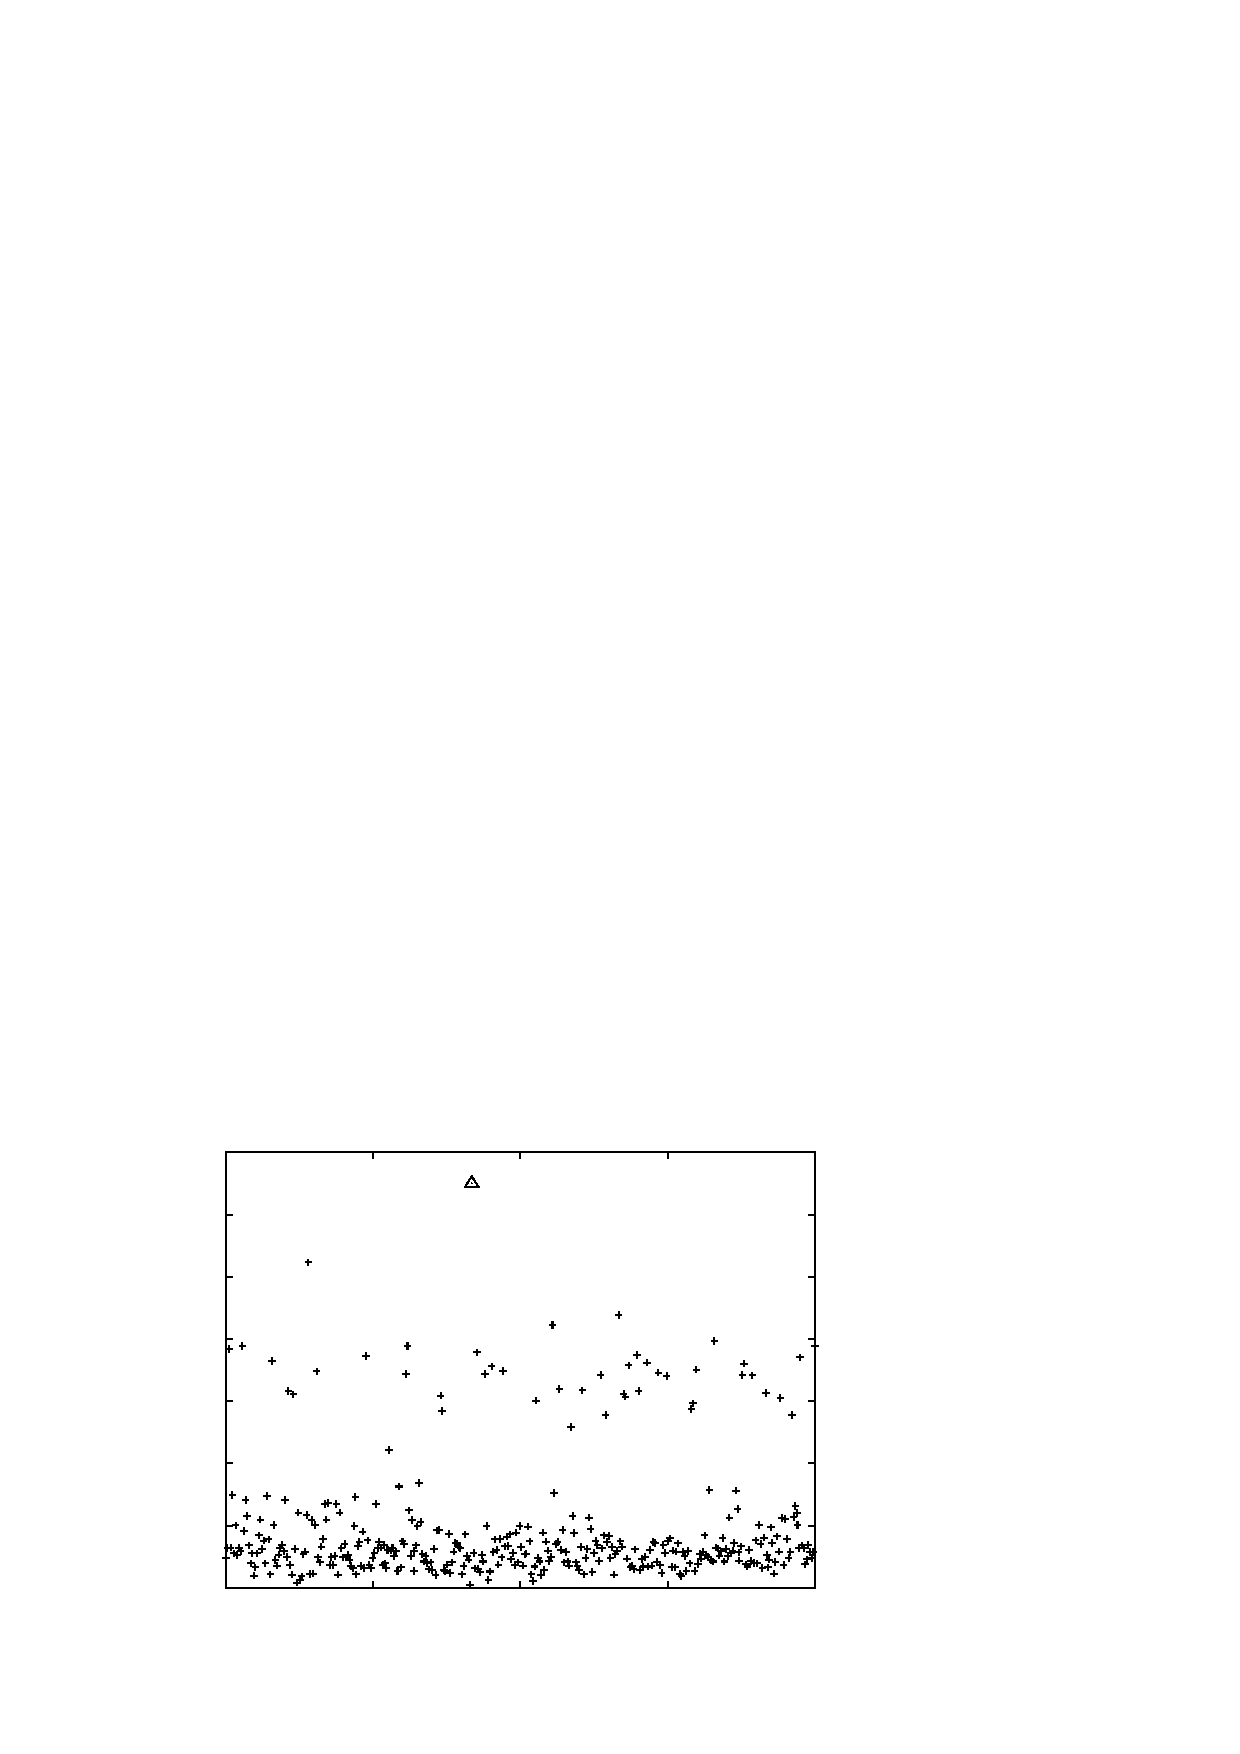
\includegraphics{fig/preTotSchedND.pdf}}%
    \gplfronttext
  \end{picture}%
\endgroup
}}}  \vspace{14pt}%
 
 \subfloat[\small{\textbf{Linux$^{\mathbf{Xen}}$ - without load} \newline
   \vskip 1mm M: 2.1, SD: 0.5, Mn: 1.8, Mx: 8.4}]{%
   \label{fig:xenSemSched}%
   {\scalebox{0.67}{\input{fig/xenSemSched}}}} \hspace{10pt}%
 \subfloat[\small{\textbf{Linux$^{\mathbf{Xen}}$ - with load} \newline
   \vskip 1mm M: 8.7, SD: 0.3, Mn: 1.8, Mx: 18.7}]{%
   \label{fig:xenTotSched}%
   {\scalebox{0.67}{\input{fig/xenTotSched}}}}  \vspace{14pt}%

 \caption[]{Activation latencies.  The $eth_0$ interrupt handler is triggered
     by packets arriving at a $20 Hz$ frequency.}
 \label{fig:latAtiv}%
\end{figure*}

\begin{figure*}[t]%
 \centering
 \subfloat[\small{\textbf{Linux$^{\mathbf{Xen}}$ - Interrupt latency - without load} \newline
 \vskip 1mm M:    9.1, SD:     0.3,  Mn:    9.8, Mx:    13.4  }]{%
   \label{fig:xenSem2}%
   {\scalebox{0.67}{\input{fig2/xenSem}}}} \hspace{10pt}%
 \subfloat[\small{\textbf{Linux$^{\mathbf{Xen}}$ - Interrupt latency - with load} \newline
 \vskip 1mm M:    11.3, SD:     1.2,  Mn:    9.0, Mx:    19.7 }]{%
   \label{fig:xenTot2}%
   {\scalebox{0.67}{\input{fig2/xenTot}}}}%

 \subfloat[\small{\textbf{Linux$^{\mathbf{Xen}}$ - Activation latency - without load} \newline
 \vskip 1mm M:     4.0, SD:     0.3,  Mn:     0.3, Mx:     9.6 }]{%
   \label{fig:xenSemSched2}%
   {\scalebox{0.67}{\input{fig2/xenSemSched}}}} \hspace{10pt}%
 \subfloat[\small{\textbf{Linux$^{\mathbf{Xen}}$ - Activation latency - with load} \newline
 \vskip 1mm M:     9.8, SD:     2.0,  Mn:     2.7, Mx:    20.8 }]{%
   \label{fig:xenTotSched2}%
   {\scalebox{0.67}{\input{fig2/xenTotSched}}}}

 \caption[Activation latencies]{Linux$^{\mathbf{Xen}}$ latencies. Interrupt requests
   at $S_M$ are triggered at a $20 Hz$ frequency by $S_T$.}
 \label{fig:latIrqAtiv2}%
\end{figure*}


By analyzing the values of activation latencies of Linux$^{\mathbf{PrtND}}$, 
it can be noticed that those values are acceptable when compared to
Linux$^{\mathbf{Prt}}$ in the absence of load. 
Nonetheless, the results obtained in load scenarios still indicate a slight
less predictable behavior than Linux$^{\mathbf{Xen}}$.

\subsection{Second Experiment}
\label{sec:results-2}

As will be seen, the timing patterns obtained by the second experiment were similar
to those described in the previous section. In order to avoid repeating the
illustration of such patterns, we summarized these results in Table
\ref{tab:dataSetUp}, which is presented in Section \ref{sec:compTable}.

Before presenting these results, though, we first illustrate the differences between
both types of experiments. To do so, we discuss the results regarding
Linux$^{\mathbf{Xen}}$ only. This platform serves well for our illustration purposes
because: (i) the results of the first experiment have indicated that
Linux$^{\mathbf{Xen}}$ is more predictable than the other platforms; (ii) station
$S_T$ was configured to use Linux$^{\mathbf{Xen}}$.  The results for
Linux$^{\mathbf{Xen}}$ are plotted in Figure \ref{fig:latIrqAtiv2} and will be
discussed in Sections \ref{sec:latIrq} and \ref{sec:latAtiv}.

%\pagebreak
\subsubsection*{Interrupt latencies in Linux$^{\mathbf{Xen}}$}
\label{sec:latIrq}

According to the experiment setup, the measurements are carried out by station $S_T$
(as shown by Figure \ref{fig:dispExp2}). As explained in Section \ref{sec:exp2},
there is an extra delay $\delta$ that must be considered in the measurements. This
delay corresponds to the value of $L_{irq}$ in $S_T$. In other words, since
Linux$^{\mathbf{Xen}}$ is being used in both stations, one expects measuring $t_2 -
t_1 = 2 \delta$ in scenarios without load. From this measurement, the value of
$\delta$, estimated through the first experiment can be confirmed. Figure
\ref{fig:xenSem2} shows the values of $L_{irq}$ minus the mean value of $\delta$,
estimated to be $9.0 \mu s$. As can be seen, these values equal $9.1 \mu s$ with a
standard deviation of $0.3$.

% Following the above discussion, in order to analyze the behavior of the system in
% load scenarios, one must take into consideration the value of $\delta$ in
% $S_T$.

Once $\delta$ is subtracted from the other results plotted in Figure
\ref{fig:xenTot2}, it can be seen that the system behaves very similarly to the
first experiment.  A noticeable difference is a significant increase of the standard
deviation. This can be explained as follows. In the first experiment, ISR$_{eth_0}$
issues an interrupt request and then finishes its execution. The pending interrupt
is immediately detected and the execution of the associated handler begins with a
minimum delay since the indirection scheme of the Adeos nanokernel guarantees that
no other interruption can delay the start of ISR$_{PP}$. Such scenarios do not occur
in the second experiment since the parallel port interrupts are externally triggered
by $S_T$. Therefore, possible interference in the interrupt handler execution can be
caused by context-switching overhead. As a result, the second experiment captures
actual scenarios of interrupt latencies more accurately, as can be seen from the
higher variability of the obtained results.

%%%
% Paul' comment:
% Values of interrupt latency are those obtained by subtracting \delta = 9.0 us.
%
 
\newcommand{\cspc}{@{\hspace{0.23cm}}}
\begin{table*}[t!]
\centering
\caption{Latency results in $\mu s$ for Linux$^{\mathbf{Std}}$, Linux$^{\mathbf{Prt}}$,
  Linux$^{\mathbf{PrtND}}$ %(option IRQF\_NODELAY) 
  and Linux$^{\mathbf{Xen}}$ using
  Experiments 1 and 2. \vspace{0.3cm}}
 \label{tab:dataSetUp}
{\scalebox{1}{
\begin{tabular}{p{0.4cm} @{} p{0.9cm}
|r \cspc r | r \cspc r | r \cspc r | r \cspc r | r \cspc r | r \cspc r | r \cspc r | r \cspc r |}
\cline{3-18}

&&
\multicolumn{4}{|c|}{\rule{0cm}{0.5cm}Linux$^{\mathbf{Std}}$}&
\multicolumn{4}{|c|}{Linux$^{\mathbf{Prt}}$}&
\multicolumn{4}{|c|}{Linux$^{\mathbf{PrtND}}$}&
\multicolumn{4}{|c|}{Linux$^{\mathbf{Xen}}$}\\

\cline{2-18}
&
\vline \rule{0cm}{0.37cm} Load &
\multicolumn{2}{|c|}{no}&
\multicolumn{2}{|c|}{yes}&
\multicolumn{2}{|c|}{no}&
\multicolumn{2}{|c|}{yes}&
\multicolumn{2}{|c|}{no}&
\multicolumn{2}{|c|}{yes}&
\multicolumn{2}{|c|}{no}&
\multicolumn{2}{|c|}{yes}\\
\cline{2-18}

&&
\rule{0cm}{0.35cm}$\mathbf{L_{irq}}$ & $\mathbf{L_{act}}$ & 
$\mathbf{L_{irq}}$ & $\mathbf{L_{act}}$ & $\mathbf{L_{irq}}$ & $\mathbf{L_{act}}$ &
$\mathbf{L_{irq}}$ & $\mathbf{L_{act}}$ & $\mathbf{L_{irq}}$ & $\mathbf{L_{act}}$ &
$\mathbf{L_{irq}}$ & $\mathbf{L_{act}}$ & $\mathbf{L_{irq}}$ & $\mathbf{L_{act}}$ &
$\mathbf{L_{irq}}$ & $\mathbf{L_{act}}$\\
\cline{2-18}

\multirow{4}{*}{\begin{sideways}\textbf{Exp. 1}\rule{0.1cm}{0.cm}\end{sideways}}
&
\vline \rule{0cm}{0.35cm} Mean &
  8.9 &  4.6 & 10.4 & 37.3 & 21.5 &  2.1 & 58.5 & 3.8 &
 8.9 &  5.3 & 10.6 &   8.0 &   9.0 &  2.1 & 10.2 & 8.7\\
\cline{2-18}

&
\vline \rule{0cm}{0.35cm} SD &
 0.3 &  0.4 &  1.9 & 48.2 &  1.7 &  0.2 & 26.4 & 2.8 &
 0.2 &  0.3 &  1.6 & 2.0 &   0.1 &   0.5 &   0.1 & 0.3\\
\cline{2-18}

&
\vline \rule{0cm}{0.35cm} Min &
  8.7 &  4.4 &  8.8 &  4.6 & 20.3 &  1.2 & 17.2 & 1.1 &
  8.8 &  5.0 &  8.9 &  5.2 &   8.8 &  1.8 &   8.8 & 1.8\\
\cline{2-18}

&
\vline \rule{0cm}{0.35cm} Max &
18.4 & 16.2 & 67.7 & 617.5 & 45.1 & 9.4 & 245.9 & 27.4 &
16.7 & 13.1 & 35.8 & 31.0 & 11.1 & 8.4 & 20.8 & 18.7\\
%\cline{2-18}
\hline\hline\hline
%\cline{2-18}
\multirow{4}{*}{\begin{sideways}\textbf{Exp. 2}\rule{0.1cm}{0.cm}\end{sideways}}
&
\vline \rule{0cm}{0.35cm} Mean &
   9.0 &  3.6  & 12.5   & 19.9 &
 10.2 &  3.7  & 31.2   &  7.2  &
   9.2 &  4.6  & 11.8   & 14.9 &
   9.1 &  4.0  & 11.3   &  9.8  \\
\cline{2-18}

&
\vline \rule{0cm}{0.35cm} SD &
  0.4 &  0.6 &  3.2 & 17.4 &
  0.5 &  0.4 & 19.0 &  3.1 &
  0.4 &  0.5 &  2.3 &  5.6  & 
  0.3 &  0.3 &  1.2 &  2.0  \\
\cline{2-18}

&
\vline \rule{0cm}{0.35cm} Min &
    8.8 & -1.3 &    9.0 &  2.3 &
  10.0 &  0.8 &  10.4 &  2.2 &
    8.9 &  -0.3 &    9.1 &  4.5 & 
    8.8 &  0.3 &    9.0 &  2.7 \\
\cline{2-18}

&
\vline \rule{0cm}{0.35cm} Max &
  18.4 & 19.0 &   75.0 & 428.4  & 
  30.8 & 12.7 & 203.9 &   21.2  &
  14.9 & 14.2 &   49.2 &   85.0  &
  13.4 &  9.6  &   19.7  &  11.8  \\
\cline{2-18}
\cline{2-18}

\end{tabular}
}} % End scalebox
\end{table*}

\subsubsection*{Activation latencies in Linux$^{\mathbf{Xen}}$}
\label{sec:latAtiv}

Two aspects must be considered when measuring activation latencies by the second
experiment (as shown by Figure \ref{fig:dispExp2}). Both aspects are dealt with by
our experiment set-up.

First, as mentioned earlier, the interrupt request issued by $\tau$ may take place
before or after $t_2$, turning the value of $t_3 - t_2$ into an imprecise
measurement. For example, if $\tau$ issues an interrupt request at $S_T$ before
$t_2$, this request will be triggered before the handling of the pending interrupt
requested by ISR$_{PP}$ at $S_T$. Thus, these two requests will be handled in a row,
which makes the value of $t_3- t_2$ too short. On the other hand, if the interrupt
request by $\tau$ takes place after $t_2$, as represented in Figure
\ref{fig:dispExp2}, this undesirable interference disappears and $t_3 - t_2$ turns
to be an accurate measurement of $L_{irq}$. In order to circumvent this measurement
problem, an extra and constant delay of $\Delta = 10 \mu s$ was introduced so that
the interrupt request issued by $\tau$ always takes place after $t_2$.

The second aspect is due to the interrupt latency variability at $S_T$. As this
station runs Linux$^\mathbf{Xen}$, it was seen in the first experiment that $L_{irq}
\in [8.8,11.1]$ when no load scenarios are considered. This means that when
measuring $L_{act}$, one can obtain values $(t_3 - t_2) \pm 2.3 \mu s$ in worst
case.

The graphs in Figure \ref{fig:xenSemSched2} show the activation latencies obtained
by the described approach. The values are already subtracted by $10 \mu s$ and so
they correspond to the measured values of $L_{act}$. The obtained values in
the graphs are very close to the ones obtained by the first experiment as can be
seen by the small differences between the mean values. Also, as expected, the variability
is now higher due to the way the experiment was set up.

%\newpage
\subsection{Comparative Analysis}
\label{sec:compTable}

Table \ref{tab:dataSetUp} summarizes the results regarding all analyzed platforms.
Both types of experiments are reported. As can be seen, their results can be used
for comparing the platform behaviors using either experiment, as mentioned before.

As expected, the data obtained for Linux$^\mathbf{Std}$ indicate that it is not
suitable to deal with real-time systems. Load scenarios make the interrupt and
activation latencies much larger than the observed mean values.

As observed before, the way Linux$^\mathbf{Prt}$ deals with interrupt request may
cause excessive delays in interrupt latencies in load scenarios. This behavior is
verified in both experiments. When option \cod{IRQF\_NODELAY} is used, the
obtained values show a behavior similar to Linux$^\mathbf{Std}$ in both experiments,
although Linux$^\mathbf{PrtND}$ seems much efficient.

It is interesting to notice that there have been negative values of activation
latencies as for the second experiment.  This can be explained by the variability of
$\delta$ at station $S_T$ (recall section \ref{sec:latIrq}).  For example, consider
that $\delta \in [\delta_{min},\delta_{max}]$. Also, recall that there is a constant
delay of $\Delta$ introduced in the measurement. Hence, $t_3 - t_2 - \Delta \in
[\delta_{min}-\delta_{max},\delta_{max}-\delta_{min}]$. Since in our experiments it
was observed that $\delta_{min} = 8.8 \mu s$ and $\delta_{max} = 11.1 \mu s$, a
negative value may be found whenever the actual $L_{act} \leq 2.3 \mu s$. However,
it is important to emphasize that we rarely observed negative values during the
experiments, only once in $12\,000$ measurements.

Among the analyzed platforms Linux$^\mathbf{Xen}$ shows higher predictability levels
when compared to the other platforms. This characteristic is of paramount importance
when it comes to sup\-porting real-time systems.  It is worth emphasizing that for
such systems predictability is preferable than speed. Thus, although the mean values
obtained by Linux$^\mathbf{Prt}$ are smaller, Linux$^\mathbf{Xen}$ seems a better
alternative when predic\-tability is aimed for.

\begin{figure}[h!tb]%
 \centering
 \label{fig:histo}%
 {\scalebox{0.64}{% GNUPLOT: LaTeX picture with Postscript
\begingroup
  \makeatletter
  \providecommand\color[2][]{%
    \GenericError{(gnuplot) \space\space\space\@spaces}{%
      Package color not loaded in conjunction with
      terminal option `colourtext'%
    }{See the gnuplot documentation for explanation.%
    }{Either use 'blacktext' in gnuplot or load the package
      color.sty in LaTeX.}%
    \renewcommand\color[2][]{}%
  }%
  \providecommand\includegraphics[2][]{%
    \GenericError{(gnuplot) \space\space\space\@spaces}{%
      Package graphicx or graphics not loaded%
    }{See the gnuplot documentation for explanation.%
    }{The gnuplot epslatex terminal needs graphicx.sty or graphics.sty.}%
    \renewcommand\includegraphics[2][]{}%
  }%
  \providecommand\rotatebox[2]{#2}%
  \@ifundefined{ifGPcolor}{%
    \newif\ifGPcolor
    \GPcolorfalse
  }{}%
  \@ifundefined{ifGPblacktext}{%
    \newif\ifGPblacktext
    \GPblacktextfalse
  }{}%
  % define a \g@addto@macro without @ in the name:
  \let\gplgaddtomacro\g@addto@macro
  % define empty templates for all commands taking text:
  \gdef\gplbacktext{}%
  \gdef\gplfronttext{}%
  \makeatother
  \ifGPblacktext
    % no textcolor at all
    \def\colorrgb#1{}%
    \def\colorgray#1{}%
  \else
    % gray or color?
    \ifGPcolor
      \def\colorrgb#1{\color[rgb]{#1}}%
      \def\colorgray#1{\color[gray]{#1}}%
      \expandafter\def\csname LTw\endcsname{\color{white}}%
      \expandafter\def\csname LTb\endcsname{\color{black}}%
      \expandafter\def\csname LTa\endcsname{\color{black}}%
      \expandafter\def\csname LT0\endcsname{\color[rgb]{1,0,0}}%
      \expandafter\def\csname LT1\endcsname{\color[rgb]{0,1,0}}%
      \expandafter\def\csname LT2\endcsname{\color[rgb]{0,0,1}}%
      \expandafter\def\csname LT3\endcsname{\color[rgb]{1,0,1}}%
      \expandafter\def\csname LT4\endcsname{\color[rgb]{0,1,1}}%
      \expandafter\def\csname LT5\endcsname{\color[rgb]{1,1,0}}%
      \expandafter\def\csname LT6\endcsname{\color[rgb]{0,0,0}}%
      \expandafter\def\csname LT7\endcsname{\color[rgb]{1,0.3,0}}%
      \expandafter\def\csname LT8\endcsname{\color[rgb]{0.5,0.5,0.5}}%
    \else
      % gray
      \def\colorrgb#1{\color{black}}%
      \def\colorgray#1{\color[gray]{#1}}%
      \expandafter\def\csname LTw\endcsname{\color{white}}%
      \expandafter\def\csname LTb\endcsname{\color{black}}%
      \expandafter\def\csname LTa\endcsname{\color{black}}%
      \expandafter\def\csname LT0\endcsname{\color{black}}%
      \expandafter\def\csname LT1\endcsname{\color{black}}%
      \expandafter\def\csname LT2\endcsname{\color{black}}%
      \expandafter\def\csname LT3\endcsname{\color{black}}%
      \expandafter\def\csname LT4\endcsname{\color{black}}%
      \expandafter\def\csname LT5\endcsname{\color{black}}%
      \expandafter\def\csname LT6\endcsname{\color{black}}%
      \expandafter\def\csname LT7\endcsname{\color{black}}%
      \expandafter\def\csname LT8\endcsname{\color{black}}%
    \fi
  \fi
  \setlength{\unitlength}{0.0500bp}%
  \begin{picture}(7200.00,5040.00)%
    \gplgaddtomacro\gplbacktext{%
      \csname LTb\endcsname%
      \put(1166,660){\makebox(0,0)[r]{\strut{} 1}}%
      \put(1166,1346){\makebox(0,0)[r]{\strut{} 10}}%
      \put(1166,2032){\makebox(0,0)[r]{\strut{} 100}}%
      \put(1166,2718){\makebox(0,0)[r]{\strut{} 1000}}%
      \put(1166,3404){\makebox(0,0)[r]{\strut{} 10000}}%
      \put(1166,4090){\makebox(0,0)[r]{\strut{} 100000}}%
      \put(1166,4776){\makebox(0,0)[r]{\strut{} 1e+06}}%
      \put(1298,440){\makebox(0,0){\strut{} 0}}%
      \put(2554,440){\makebox(0,0){\strut{} 5}}%
      \put(3811,440){\makebox(0,0){\strut{} 10}}%
      \put(5067,440){\makebox(0,0){\strut{} 15}}%
      \put(6323,440){\makebox(0,0){\strut{} 20}}%
      \put(356,2718){\rotatebox{90}{\makebox(0,0){\strut{}Number of events}}}%
      \put(4062,110){\makebox(0,0){\strut{}Time $\mu s$}}%
    }%
    \gplgaddtomacro\gplfronttext{%
      \csname LTb\endcsname%
      \put(5839,4603){\makebox(0,0)[r]{\strut{}$L_{act}$}}%
      \csname LTb\endcsname%
      \put(5839,4383){\makebox(0,0)[r]{\strut{}$L_{irq}$}}%
    }%
    \gplbacktext
    \put(0,0){\includegraphics{fig/histo}}%
    \gplfronttext
  \end{picture}%
\endgroup
}} \hspace{10pt}%
 \caption{1,000,000 events histogram for Linux$^\mathbf{Xen}$. Each histogram, log-scaled,
 corresponds to the number of events in the $1 \mu s$ interval beginning
 at the corresponding x-value.
 %where the x-axis indicates the lower value of such intervals.
}
\end{figure}

Since Linux$^\mathbf{Xen}$ presented the best results in our previous experiments,
we decided to run the second experiment during a longer period to see how stable
this system would be. Thus, we ran the second experiment for 14 hours with the same
load scenarios presented earlier. This setup generated more than 1 million events.
The histogram of Figure \ref{fig:histo} presents the number of events per activation
and interrupt latencies in 1 $\mu s$ steps on a logarithmic scale. From this figure,
we see that over $100,000$ events had both activation and interrupt latencies within
$[10, 11]$ $\mu s$. Although some worst-case latencies are greater than those
observed in the corresponding 10-minute experiments, these were very rare events.

\section{Related work}
\label{sec:trabRel}

Some experimental results comparing Linux$^{\mathbf{Prt}}$ and
Linux$^{\mathbf{Std}}$ are presented in \cite{Rostedt07}. They measured interrupt
and scheduling latencies of a periodic task. However, their experiments were
conducted without processor load and the methodology used was not precisely
described. Siro et al \cite{Siro07} compares Linux$^{\mathbf{Prt}}$, RT-Linux
\cite{Barabanov97} and Linux$^{\mathbf{RTAI}}$ \cite{Dozio03} with LMbench
\cite{McVoy96} by measuring the scheduling deviation of a periodic task. The authors
tested the systems with a load overhead, but they did not consider interrupt
load. In their website, the developers of the Adeos project \cite{Benoit05} present
some comparative results for \preemptt and Adeos. In their evaluation, they used
LMbench \cite{McVoy96} to characterize the performance of the two platforms and
measured the interrupt latencies gathered from the parallel port.

The interrupt latency results of our work are similar to those obtained by Benoit et
al \cite{Benoit05} for Linux$^{\mathbf{Xen}}$. However, our results differ from
their work for Linux$^{\mathbf{Prt}}$ since we noticed some degradation of time
guarantees by this platform, as reported in Sections \ref{sec:latIrq} and
\ref{sec:compTable}.  Regarding activation latencies under load scenarios, we are
not aware of any other comparative work. Experiments similar to those reported here
were conducted for Linux$^{\mathbf{RTAI}}$ \cite{Regnier08c}. As expected, the obtained results are
similar to those presented for Linux$^{\mathbf{Xen}}$, since both platforms use
Adeos nanokernel. 
% Some of the results presented in this paper have recently been
% discussed in a local forum \cite{Regnier08-wso}.

\section{Conclusion}
\label{sec:conc}

In this work, we have conducted a comparative evaluation of two Linux-based
RTOS. Our comparative methodology has allowed experimental
measurements of interrupt and activation latencies in scenarios of variable
load. Load of both processing and those due to interrupt handling have been
considered. Two experiments have been defined.  In the simpler one, the
same station that deals with real-time activities is responsible for the
measurements. In the second, the measurements are carried out externally, by a
different station. Both experiments can be used for comparison purposes although the
second one gives the values of interrupt latencies more accurately.

While standard Linux presented latencies in the worst case over $100 \mu s$, the
platforms Linux$^{\mathbf{Prt}}$ and Linux$^{\mathbf{Xen}}$ managed to provide
temporal guarantees with a precision below $20 \mu s$. However, in order to achieve
this behavior with Linux$^{\mathbf{Prt}}$, it was necessary to disable the
interruption threading for the parallel port interrupt line, making the system less
flexible. With a threaded implementation, the behavior of Linux$^{\mathbf{Prt}}$
suffers considerable deterioration of its temporal predictability.
Linux$^{\mathbf{Xen}}$ was found more appropriate since offers a user-mode
programming environment as well as better temporal predictability, a desirable
characteritic for supporting real-time systems.


\section*{Acknowledgments}

This work has received funding support from the Brazilian funding agencies CNPq
(Grant number 475851/2006-4) and FAPESB (Grant number 7630/2006).  The authors would
like to thank the anonymous reviewers whose comments helped to improve the quality
of this paper.

\bibliographystyle{abbrv}
\bibliography{bib}

\end{document}



\begin{table}[thb]
  \centering
  \caption{Histogram}
  \label{tab:histo}
  {\scalebox{1}{
  \begin{tabular}{r r r}
    0 &                 0 &                  2 \\
    1 &                 0 &                  1 \\
    2 &                 0 &                16 \\
    3 &                 0 &                62 \\
    4 &                 0 &          32013 \\
    5 &                 0 &        146784 \\
    6 &                 0 &        108252 \\
    7 &                 0 &          43161 \\
    8 &             165 &          92108 \\
    9 &       130691 &        267450 \\
   10 &      484114 &        202462 \\
   11 &      294222 &          37629 \\
   12 &        43047 &          10336 \\
   13 &        18373 &          23463 \\
   14 &        18071 &          30459 \\
   15 &        15784 &          12061 \\
   16 &          3036 &            1220 \\
   17 &            280 &              241 \\
   18 &            108 &              111 \\
   19 &              67 &              118 \\
   20 &              33 &                48 \\
   21 &                9 &                  3 \\
   22 &                0 &                  0 \\
  \end{tabular}
}}
\end{table}

